\documentclass[10pt]{article}

\usepackage[margin=1in]{geometry}
\usepackage{amsmath,amsthm,amssymb}
\usepackage{graphicx}
\usepackage{subfig}
\usepackage{float}
\usepackage{wrapfig}
\usepackage{multicol}
\usepackage{booktabs}
\usepackage{hyperref}

 \hypersetup{
 	colorlinks=true,
 	linkcolor=blue,
 	filecolor=magenta,      
 	urlcolor=cyan,
 }

\setlength\parindent{0pt}

\graphicspath{ {/Users/clay/Documents/research/TGE-SP21/assignments/images/} }

\newcommand{\titler}[2]{
	\title{Assignment #1} %replace X with the appropriate number
	\author{Geosc 597-003 \\
		Techniques of Geophysical Experimentation} %if necessary, replace with your course title \\
	\date{Due: #2}
	
	\maketitle}


\begin{document}

% --------------------------------------------------------------
%                         Start here
% --------------------------------------------------------------

\titler{6}{09 April}

\section*{PID Control: LED dimmer}

It can take awhile to gain some intuition about control systems, especially PID controllers. In this activity you will build a simple PID controller with your Arduino and adjust the different gain settings to see their effects. This lab is based on a lab written by Bret Comnes and A. La Rosa at Portland State University. Their original lab activity is available on their \href{https://github.com/bcomnes/315-lab-microcontroller/blob/master/Arduino%2BPID%2BLab.pdf}{GitHub repo}.

The control system you will build tries to maintain a constant light level on a photo resistor. This is a closed-loop system since we have a feedback path. 

In our system, an LED will shine directly into the photo resistor. The setpoint of the system is adjustable with a potentiometer on the board. The gains of the controller can be changed using the serial interface.  \\ 

\noindent \textbf{Materials:}
\begin{multicols}{2}
	{\small \begin{itemize}
		\item Arduino UNO
		\item USB Cable
		\item LED
		\item 330 $ \Omega $ resistor (Orange-Orange-Brown)
		\item 10k $ \Omega $ resistor (Brown-Black-Orange)
		\item Photo resistor
		\item Breadboard
		\item M/M Jumper wires
		\item Computer (Mac, Linux, Windows
	\end{itemize}}
\end{multicols}

\noindent \textbf{Tasks:}
\begin{enumerate}
	\item We could write all of the PID control code ourselves, but there is an Arduino library available with a very robust controller. Installing the library is easy. Download the library zip file from the \href{https://github.com/br3ttb/Arduino-PID-Library/archive/master.zip}{GitHub repository}. Unzip the folder and move it to the Arduino library folder. In most installations you will find this in your Documents folder: ~/Documents/Arduino/libraries. If your folder has hyphens in the name, change them to underscores. If the Arduino IDE was open, restart it. You should find new examples for the PID library in \textit{File } $ \rightarrow $ \textit{Examples} $ \rightarrow $ \textit{PID}. Have a look at the examples to get an idea of how the library works.
	\item Using the parts in your kit, build the circuit we will use shown in Figure \ref{fig:PID_cirucit}. Take a photo of your circuit and attach it to the lab report. 
	\item What are the initial values of the $ K_p $, $ K_i $, $ K_d $ gains? 
	\item What happens as you change the set point of the system using the potentiometer? 
	\item At a fixed set point, change the level of incoming light by shielding the setup with your hands and by increasing the light level using a flashlight. How fast does the system respond? 
	\item Using the serial monitor, change the gain settings by sending three numbers separated by commas. For example to set $ K_p=2 $, $ K_i=10 $, $ K_d=0 $ you would send 2,10,0. Systematically vary the $ K_i $ setting with both $ K_p $ and $ K_d $ set to zero. Describe the effect this has. Why is it so? 
	\item Set $ K_i $ to 10 and systematically increase $ K_p $ with $ K_d $ set to zero. Describe the effect this has. Why is this so? 
	\item  Set $ K_i $ to 10 and systematically increase $ K_d $ with $ K_p $ set to zero. Describe the effect this has. Why is this so? 
	\item What parameters seem to be the best for controlling the light level? Why do you think that is? 
\end{enumerate}


\newpage

\begin{figure}[ht]
	\centering
	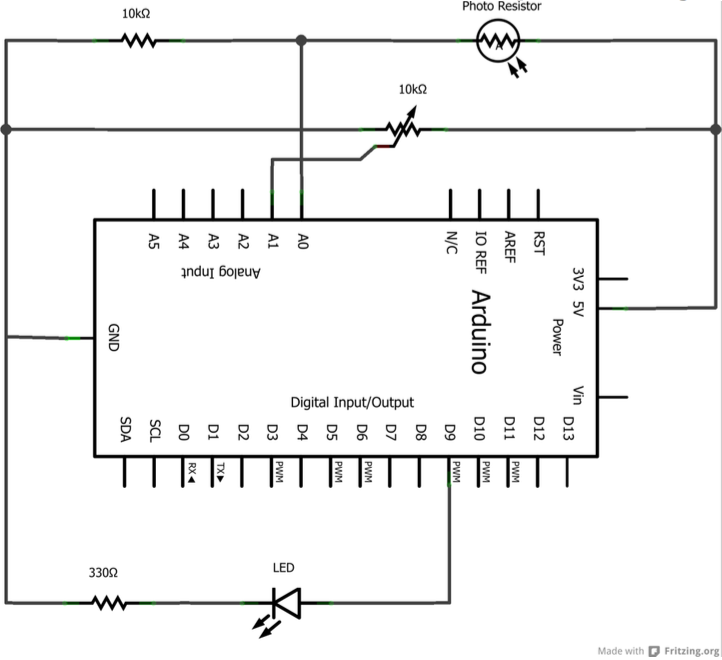
\includegraphics[width=0.8\columnwidth]{PID_circuit}
	\caption{Voltage divider circuit diagram.}
	\label{fig:PID_cirucit}
	
\end{figure}

\begin{wraptable}{r}{5cm}
	%	\begin{table}[h!t]
	\footnotesize
	\centering
	\begin{tabular}{@{}ll@{}}
		\multicolumn{2}{c}{\textbf{Grading Rubric}} \\ \midrule 
		\multicolumn{1}{l}{\textit{Topic}}   & \textit{Points}   \\ \midrule 
		answer questions  & 50   \\ \midrule
		photo of circuit   & 20   \\ \midrule
		video of working circuit & 10  \\ \midrule
		Arduino code & 20 \\ \bottomrule
	\end{tabular}
	%	\end{table}
\end{wraptable}

\section*{What to upload to Canvas}
You should upload the following with \textit{consistent file names}:

\begin{itemize}
	\item Arduino Code
	\begin{itemize}
		\item \textbf{Fully comment your code!} 
		\item Put all Arduino codes for this assignment in a project folder. 
	\end{itemize}
	\item Brief report
	\begin{itemize}
		\item Answer questions in activity.
		\item Relevant photos/figures with proper labels and brief captions.
	\end{itemize}
	\item Zip directory and upload to Canvas. (hw6\_username.zip)
\end{itemize}

\end{document}
